%%
% TUM Corporate Design LaTeX Templates
% Based on the templates from https://www.tum.de/cd
%
% Feel free to join development on
% https://gitlab.lrz.de/tum-templates/templates
% and/or to create an issue in case of trouble.
%
% tum-presentation class for scientific talks, thesis presentations, ...
%
%%

%\documentclass[4to3]{tum-presentation}
%\documentclass[navsym]{tum-presentation}
%\documentclass[nothreeliner]{tum-presentation}
%\documentclass[handout,4on1]{tum-presentation}
%\documentclass[handout,2on1]{tum-presentation}
%\documentclass[handout]{tum-presentation}
\documentclass[notes]{tum-presentation}
%%\setbeameroption{show notes on second screen=bottom}

\usepackage{natbib}
\bibliographystyle{abbrvnat}

\title[Global XAI for NLP models]{Global Explainability for Natural Language Processing Models}
\subtitle{Guided Research - Final Presentation}
\author[Simon Klimek]{B. Sc. Simon Klimek}
\institute[]{Supervisor: M. Sc. Edoardo Mosca}
\date{April 16, 2021}

\footline{\insertshortauthor~|~\insertshorttitle}

\begin{document}

\begin{frame}[noframenumbering]
  \titlepage
\end{frame}
\begin{frame}
  \frametitle{Background - eXplainable Artificial Intelligence (XAI)}
  \begin{itemize}
    \item How does a machine learning model come to a conclusion?
    \item Simple (linear) vs. complex (non-linear) models
    \item Humans can not comprehend a deep neural network!
  \end{itemize}
  \begin{columns}
  \begin{column}{.6\textwidth}
  \end{column}
  \begin{column}{.4\textwidth}
    \begin{figure}[tb]
      \centering
      
\includegraphics[width=\columnwidth]{pictures/ai.pdf}
      {\tiny illustration made by undraw.co}
    \end{figure}
  \end{column}
  \end{columns}
\end{frame}

\begin{frame}
  \frametitle{Motivation}
  \begin{itemize}
    \item First thought: What do we want to explain?
    \note{politics, hate speech, \dots}
    \item Given: A tool allowing us to search and download posts from Facebook
    
  \end{itemize}
  \vspace*{1cm}
  \only<2->{ 
  \begin{itemize}
    \item ``The idea that the current crisis may be especially fertile ground for conspiracy beliefs may well be correct.''
      \begin{itemize}
      
        \item 50\% little evidence of conspiracy thinking
        \item 25\% a degree of endorsement
        \item 15\% consistent pattern of endorsement
        \item 10\% had very high levels of endorsement
      \end{itemize}
    \only<3->{
          \item ``Higher levels of corona virus conspiracy thinking were associated with \emph{less adherence to all government guidelines} and \emph{less willingness to take diagnostic or antibody tests or to be vaccinated.}''
        }
  \end{itemize}
  }
  \only<2->{\citep{freeman_waite_etal_2020}}
  \note{ online survey with 2501 adults in England, quota sampled to match the population for age, gender, income, and region.}
\end{frame}

\begin{frame}
  \frametitle{Motivation}

  \begin{figure}[tb]
    \centering
    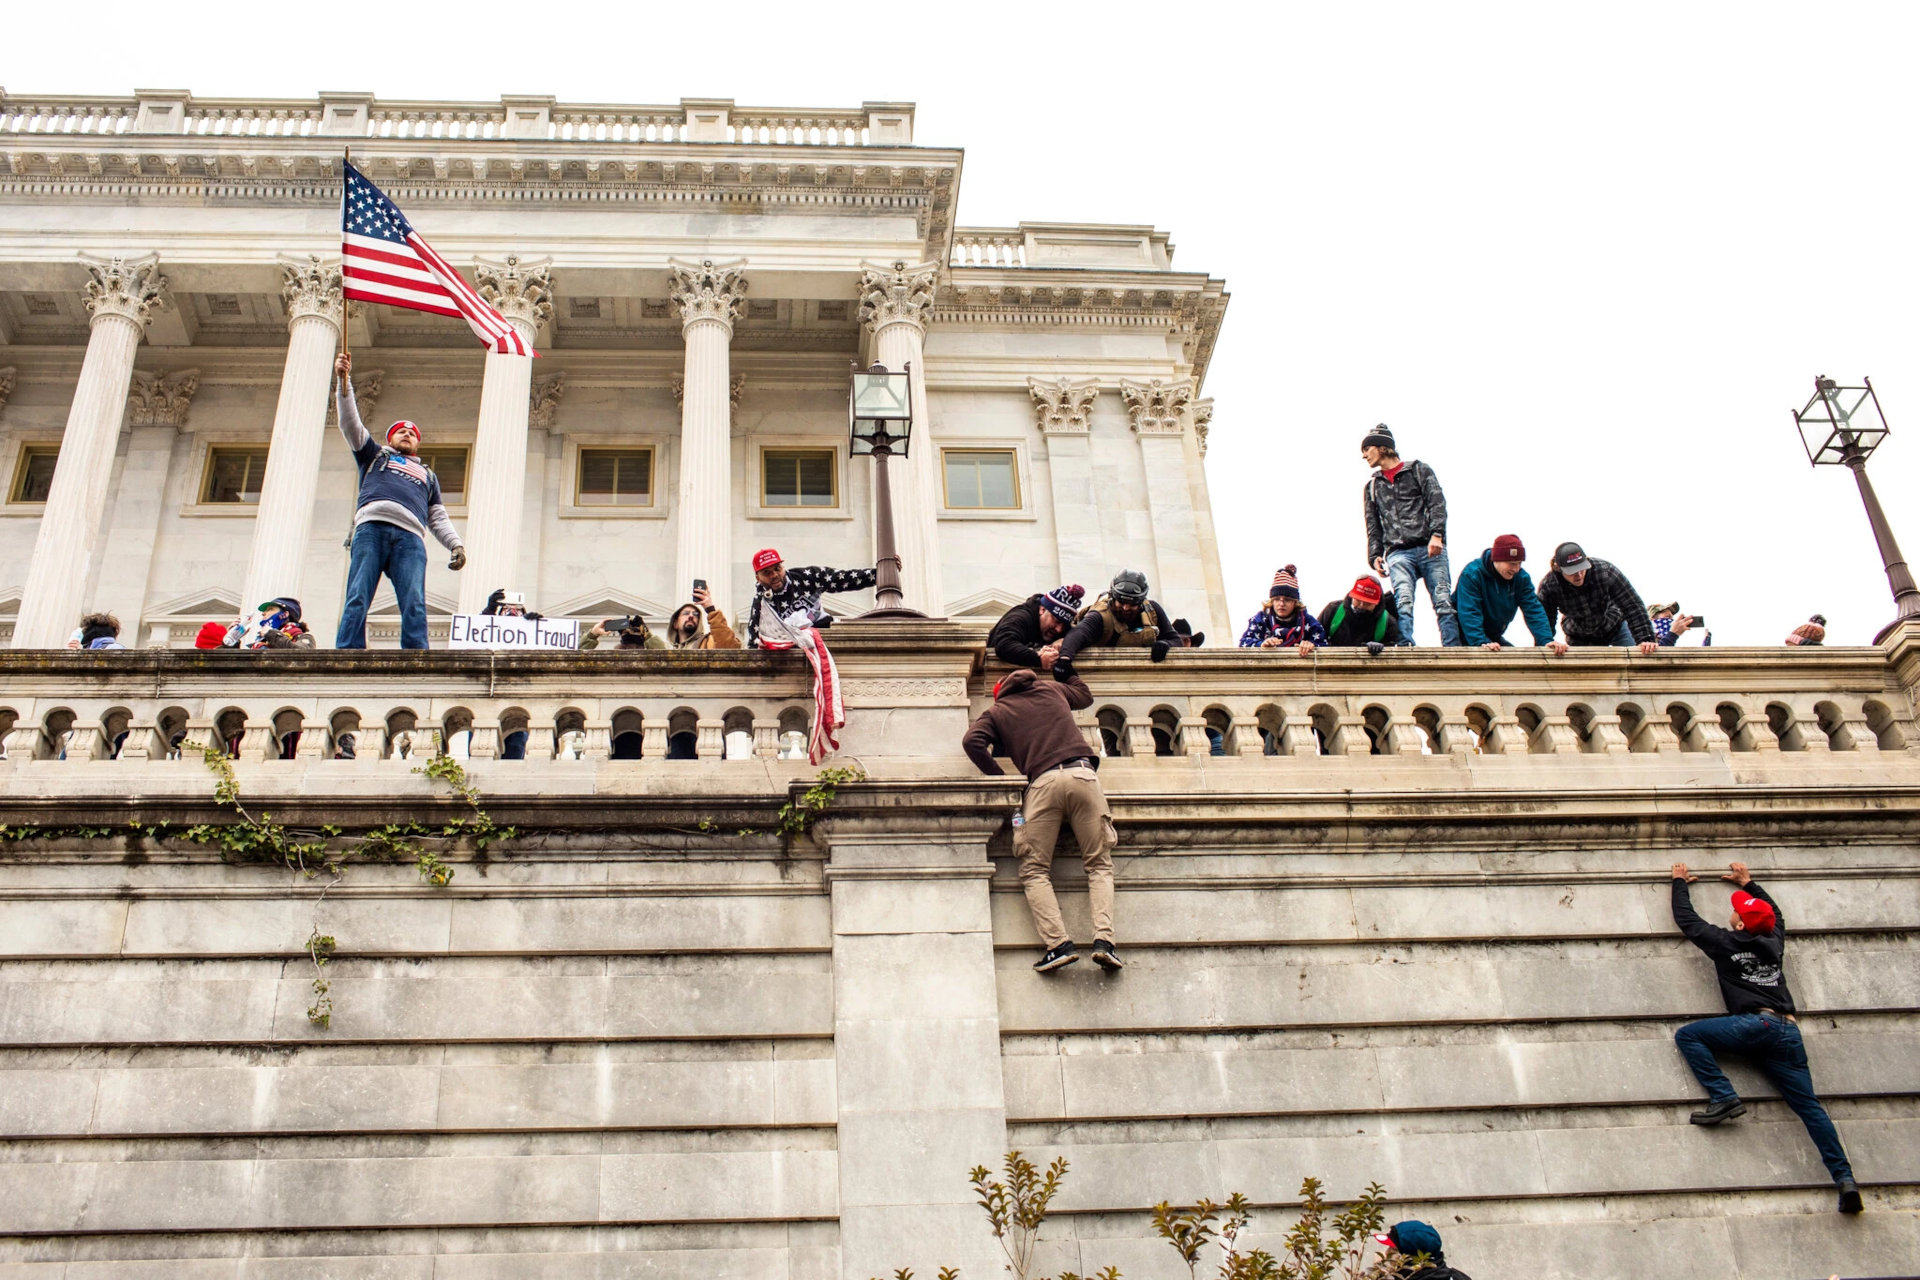
\includegraphics[width=.55\textwidth]{pictures/nytime-riots.jpg}
    \caption{Capitol Riots - Jason Andrew for The New York Times \citep{williamson_2021}}
    \label{fig:nytimes-riots}
  \end{figure}
  \note{
These theories can be  dangerous, as one can
conduct from the Capitol riot in the United States January 6th, 2021. At this event,
people believed in a conspiracy theory that Trump's victory in the US elections 2020 was 
stolen from him and tried therefore to ``take it back'' by storming the US
Capitol~\citep{williamson_2021}}.
\end{frame}




\begin{frame}
  \frametitle{Related Work}
  \citet{guidotti2018survey} - Survey giving us an overview of the state of the art XAI methods:
    
\begin{itemize}
  \item \textbf{Model Explanation Problem (global)}
  \item Outcome Explanation Problem (local)
  \item Model Inspection Problem (global/local)
  \item Transparent Box Design Problem (global/local)
\end{itemize}
\pause
\vspace*{1cm}
\begin{itemize}
  \item All global explainability methods are surrogates.
  \item Listed no global XAI methods which can be used for NLP.
  
  %% todo: maybe add palm graphics
\end{itemize}
\note {
      
  \begin{itemize}
    \item Model Explanation Problem (global)\\
    Derive an interpretable global predictor from the black box (using some
    process). -> Global Surrogate

    \item Outcome Explanation Problem (local)\\
    Derive an explanation for the prediction of a single instance using a local
    predictor.

    \item Model Inspection Problem (global/local)\\
    Provide visual or textual representation for some property of the black box
    given a set of input instances.

    \item Transparent Box Design Problem (global/local)\\
    Learning a local or global interpretable predictor using the same training
    set which was used to train the black box.
  \end{itemize}

  I.e. work on tabular data, except PALM paper
}
\end{frame}


\begin{frame}[fragile]
  \frametitle{Related Work}
  \citet{NEURIPS2020_c7bf0b7c} - Understanding Global Feature Contributions With Additive Importance Measures 
    
\begin{itemize}
  \item Based on Shapley values
  \item Not method proposed for text based inputs
  \item Uses a group of pixels for images
  \item Use a closed unit (e.g. named entity)
\end{itemize}
\pause
  \begin{columns}
  \begin{column}{.5\textwidth}
\begin{verbatim}
Here's tomorrow's Ancient Aliens lineup. Better wake
up early. Starts at 7am eastern time in the USA.
\end{verbatim}
\vspace*{.5cm}
\begin{verbatim}
The system is broken. It amazes me that a young child 
in kindergarten can be kicked out of school because a 
document isn’t checked and dated for a vaccine. We 
are all wearing masks!
\end{verbatim}
  \end{column}
  \begin{column}{.5\textwidth}
    \begin{figure}[tb]
      \centering
      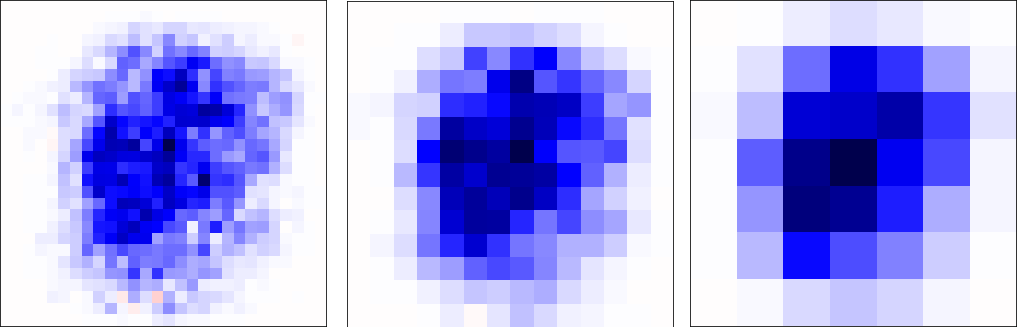
\includegraphics[width=\columnwidth]{pictures/sage-pixels.png}
      \caption{from left to right: individual pixels, 2x2 super pixels, 4x4 super pixels}
      \label{fig:figure1}
    \end{figure}
  \end{column}
  \end{columns}
\end{frame}

\begin{frame}
  \frametitle{Dataset Retrieval}
  CrowdTangle, ``a public insights tool owned and operated by Facebook''~\citep{ctshiffmanciting}

  \begin{center}
    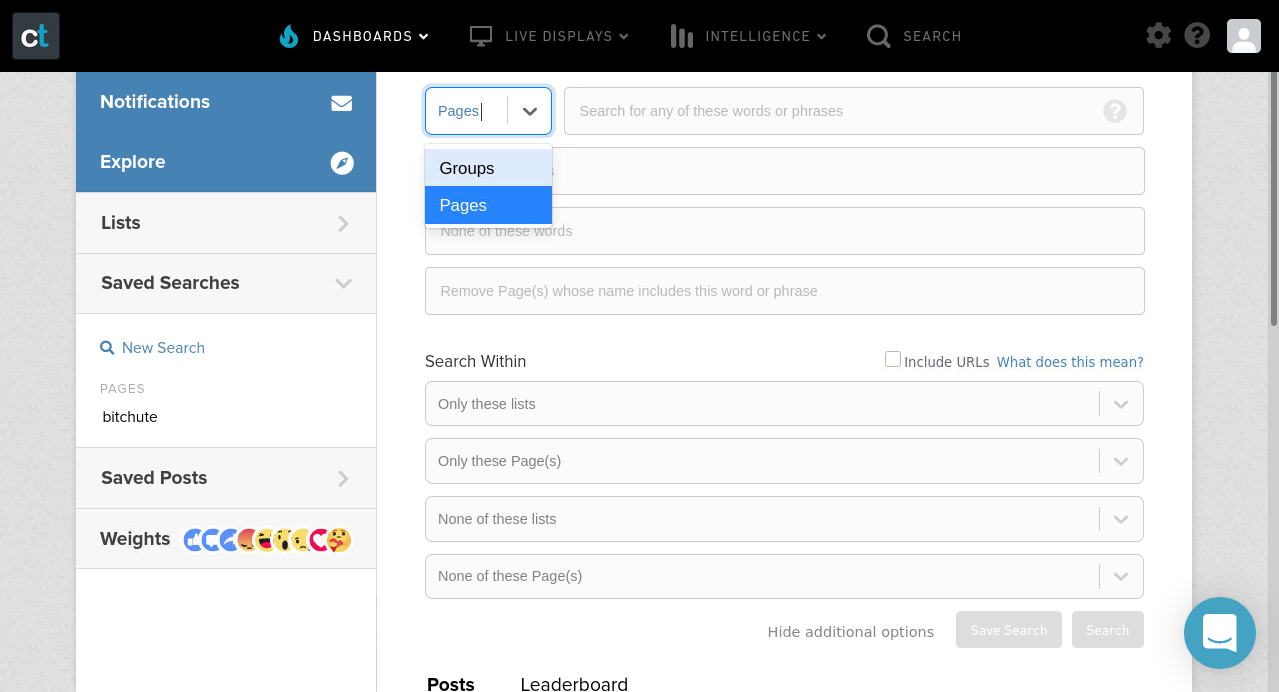
\includegraphics[width=.7\textwidth]{pictures/crowdtangle_search.png}
  \end{center}
  \note{  
  \begin{itemize}
    \item Capitol Riots, organized on social media, thus analyze social media data
    \item challenge: how can we actually find conspiracy theory groups
    \item CT: only \textbf{public} groups over 2000 members
    \item can search for a certain keyword, filter post or group
    \item How do we find conspiracy groups?? (ironic posts? just by ``accident'' (single member))
    \item Check who shared a conspiracy video

  \end{itemize}
  }
\end{frame}


\begin{frame}
  \frametitle{Dataset Retrieval}

  \begin{center}
    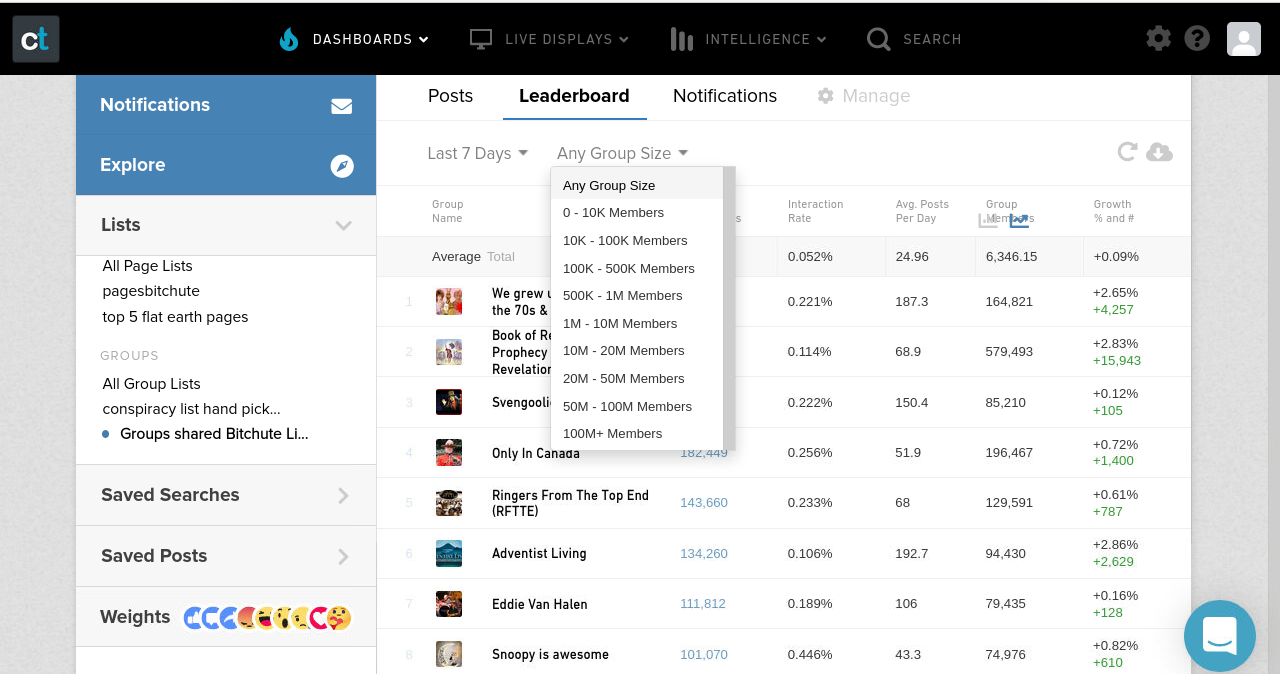
\includegraphics[width=.7\textwidth]{pictures/crowdtangle_leaderboard.png}
  \end{center}
  \note{  

  }
\end{frame}
\begin{frame}
  \frametitle{Dataset Retrieval}

  \begin{center}
    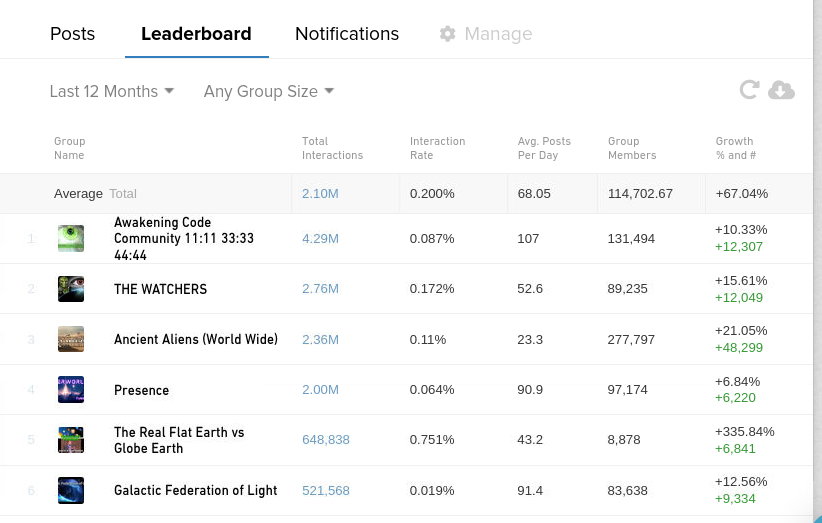
\includegraphics[width=.6\textwidth]{pictures/crowdtangle_handpicked.png}
  \end{center}
  \note{  

  }
\end{frame}
\begin{frame}
  \frametitle{Dataset Retrieval}

  \begin{center}
    
\includegraphics[width=.7\textwidth]{pictures/crowdtangle_deleted.png}
  \end{center}
  \note{  

  }
\end{frame}
\begin{frame}
  \frametitle{Dataset Retrieval}
  \begin{columns}
  \begin{column}{.5\textwidth}
      \begin{itemize}
        \item Goal: at least 30,000 posts
        \item Posts had to be at least two month old
      \end{itemize}
      \vspace*{1cm}
      \only<2->{
      \begin{itemize}
        \item Result: two datasets: conspiracy theory groups and RTnews (Russia Today)\footnotemark
      \end{itemize}
      }
  \end{column}
  \begin{column}{.5\textwidth}
  \only<2->{
    \begin{figure}[tb]
      \centering
      
\includegraphics[width=\columnwidth]{pictures/crowdtangle_rtnews.png}
      \caption{RT Facebook page}
      \label{fig:figure1}
    \end{figure}
  }
  \end{column}
  \end{columns}
  \only<2->{
    \footnotetext[1]{A paper analyzing how RT shares conspiracy theories and false information
      was written by \citet{yablokov2015conspiracy}}
  }
\end{frame}
\begin{frame}
  \frametitle{Dataset Preprocessing}
  \begin{columns}
  \begin{column}{.5\textwidth}
    \begin{itemize}
      \item Duplicate posts have been removed
      \only<3->{\item Our score formula
      \[
        \text{score} = \frac{\text{\#reactions}}{\text{\#group avg number of reactions}}
      \]}
    \end{itemize}
    \vspace*{1cm}
    \only<3->{
      \begin{center}
        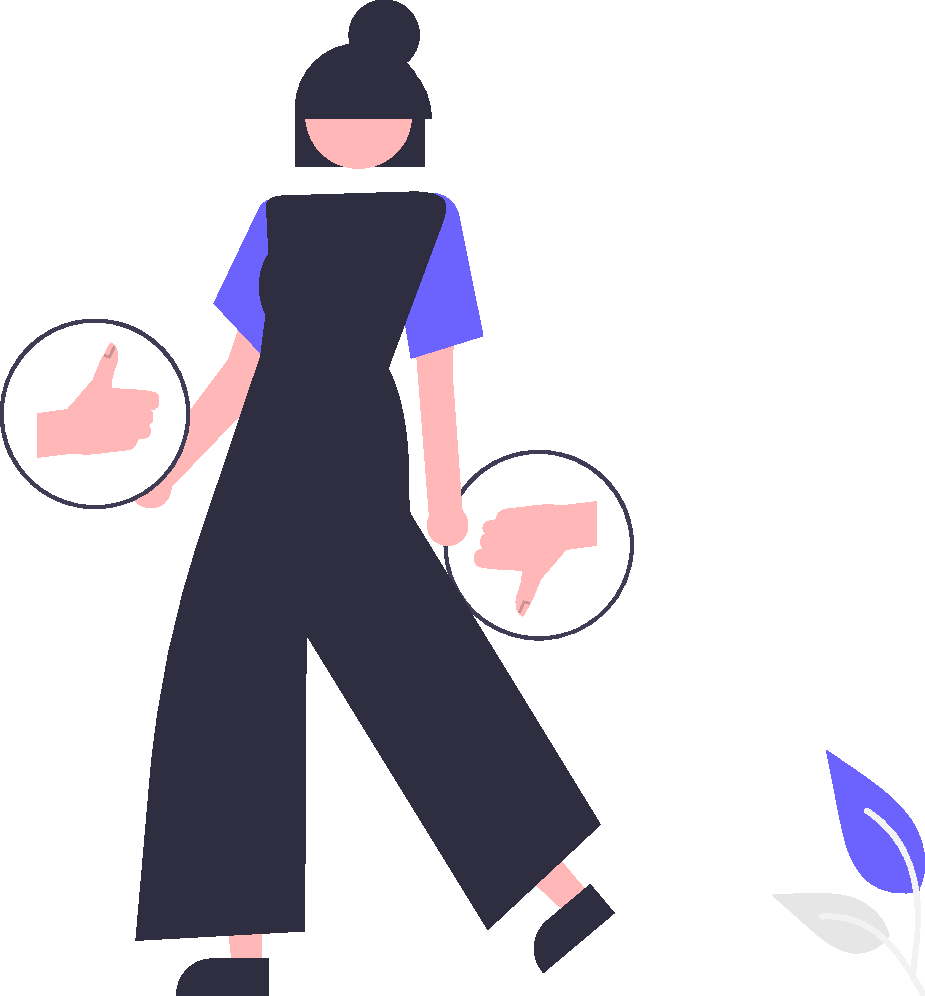
\includegraphics[width=.3\textwidth]{pictures/likedislike.pdf}\\
        {\tiny illustration made by undraw.co}
      \end{center}
    }
  \end{column}
  \begin{column}{.5\textwidth}
  \only<2->{
    \begin{figure}[tb]
      \centering
      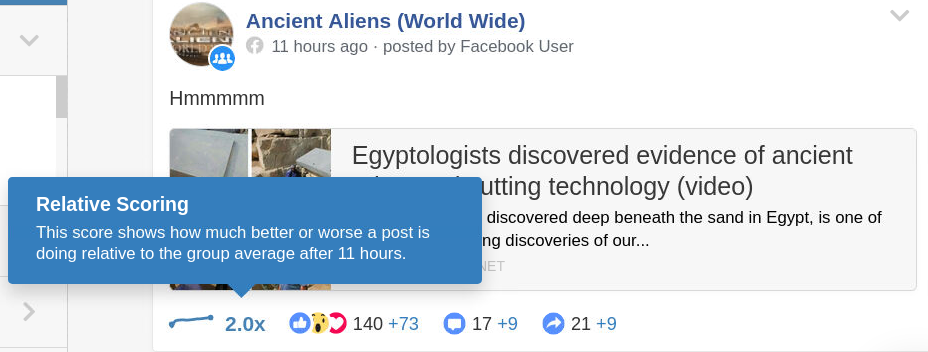
\includegraphics[width=.8\columnwidth]{pictures/crowdtangle_score.png}
      \vspace*{.5cm}\\
      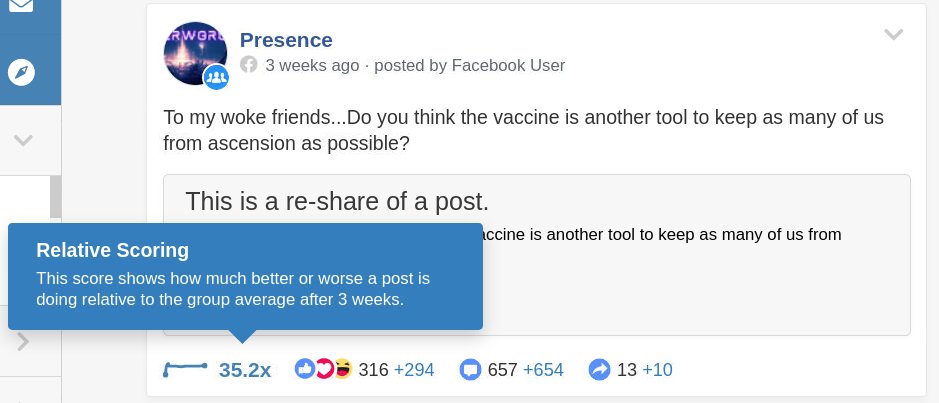
\includegraphics[width=.8\columnwidth]{pictures/crowdtangle_score2.png}
    \end{figure}
    }
  \end{column}
  \end{columns}
\end{frame}
\begin{frame}
  \frametitle{Dataset 1: Conspiracy Theory Groups}
  \begin{figure}
      \centering
      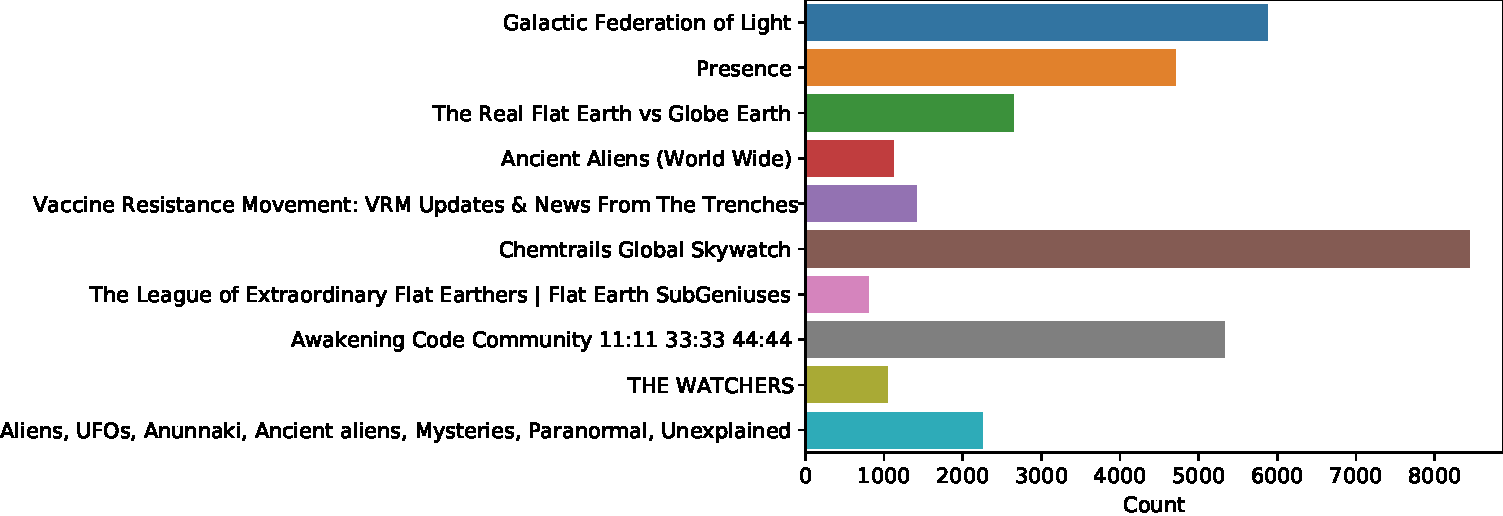
\includegraphics[width=\textwidth]{../report/figures/dataset_groups/group_dist.pdf}
  \end{figure}
  \note{
  \begin{itemize}
    \item to overcome problem of unequal distribution: group name included as feature
  \end{itemize}
  }
\end{frame}
\begin{frame}
  \frametitle{Dataset 1: Conspiracy Theory Groups}

  \begin{figure}
      \centering
      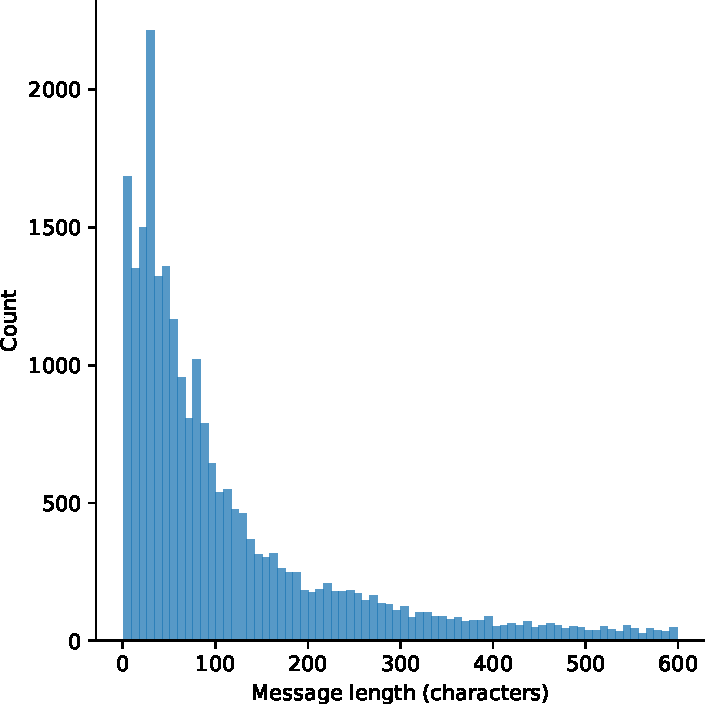
\includegraphics[width=.32\textwidth]{../report/figures/dataset_groups/message_length_dist.pdf}
      \raisebox{-0.7cm}{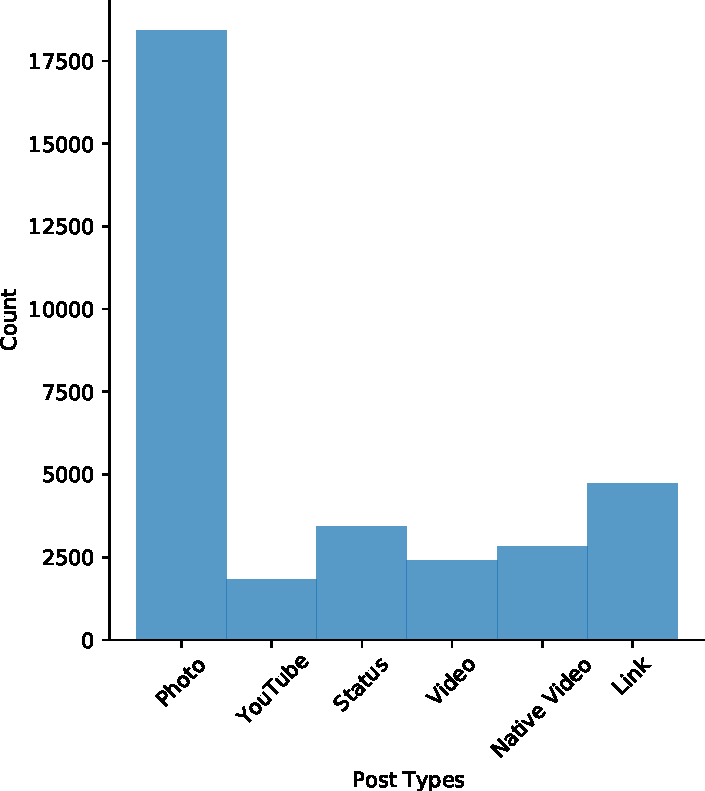
\includegraphics[width=.32\textwidth]{../report/figures/dataset_groups/post_types_dist.pdf}}
      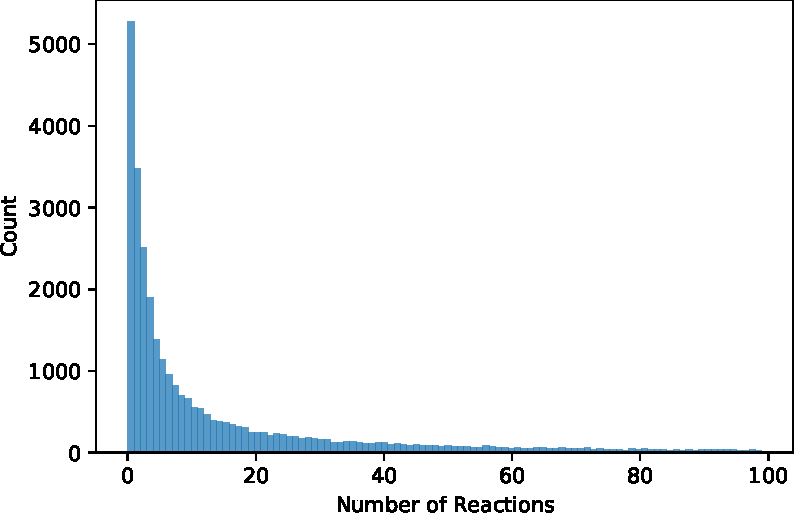
\includegraphics[width=.32\textwidth]{../report/figures/dataset_groups/reactions_dist.pdf}
  \end{figure} 
  
\end{frame}

\begin{frame}
  \frametitle{Dataset 2: rtnews}

  \begin{figure}[tb] 
    \centering
    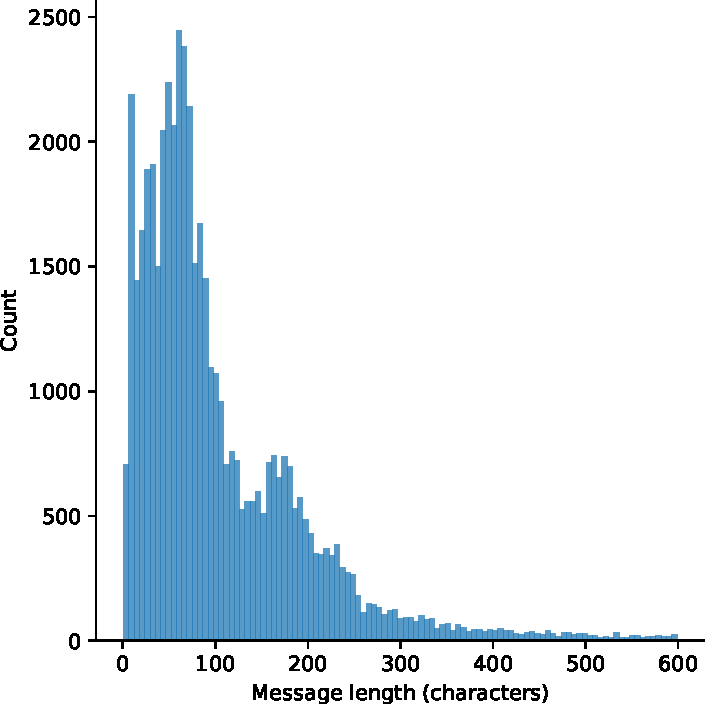
\includegraphics[width=.28\textwidth]{../report/figures/dataset_rtnews/message_length_dist.pdf}
    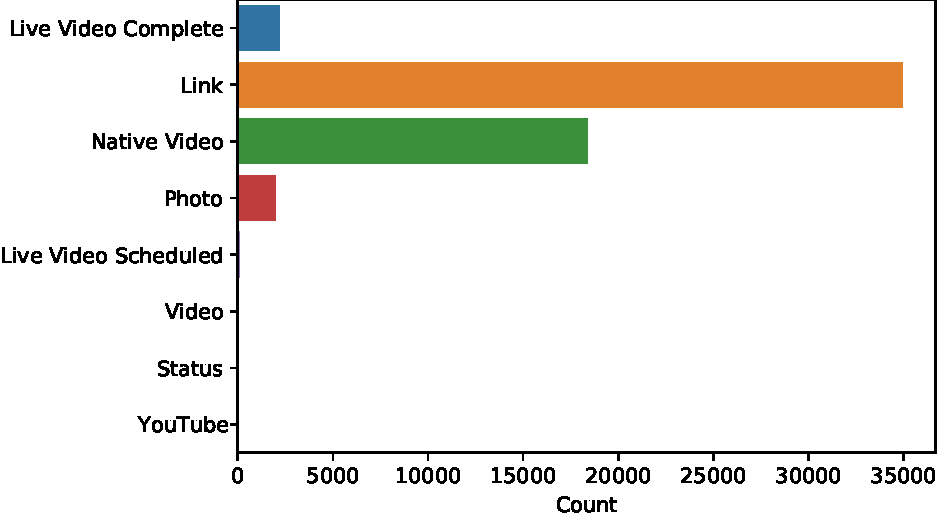
\includegraphics[width=.40\textwidth]{../report/figures/dataset_rtnews/post_types_dist.pdf}
    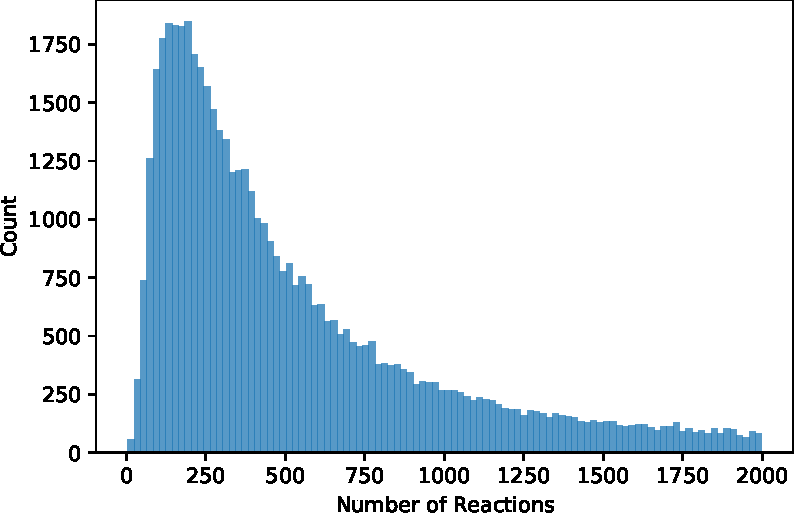
\includegraphics[width=.30\textwidth]{../report/figures/dataset_rtnews/reactions_dist.pdf}
    
    \label{fig:datasetstats-rtnews}
\end{figure} 
\end{frame}

\begin{frame}
  \frametitle{Experiments}
  \begin{columns}
  \begin{column}{.5\textwidth}
    \begin{itemize}
      \item Baseline: linear regression
      \begin{itemize}
        \item features: group, post type and top level domain
        \note{as one hot encoding, Top level domain explain extraction, 886 different top level domains}
      \end{itemize}
      \item Neural model based on DistilBert~\citep{sanh2020distilbert}
      \item BiLSTM model
      \begin{itemize}
        \item categorical features + post text
        \item optimizer: Adam
      \end{itemize}
      \item 60-20-20 split (train / validation / test)
    \end{itemize}
  \end{column}
  \begin{column}{.5\textwidth}
    %% TODO: Graphic model desc
  \end{column}
  \end{columns}
\end{frame}
\begin{frame}
  \frametitle{Results}
\begin{table}[tb]
    \caption{mean squared error for all models and datasets}
    \label{tab:results-all}
    \centering

    \begin{tabular}{l|l|l}
    \hline

    \hline
    & \textbf{conspiracy theory groups} & \textbf{rtnews}\\
    \hline
    linear model & 6.68 & 177.51\\
    \hline
    DistilBert & 6.46 & 177.00\\
    \hline
    BiLSTM & 6.54 & 177.44\\
    \hline
    \end{tabular}
\end{table}

\end{frame}

\begin{frame}
  \frametitle{Results}
\begin{table}[tb]
    \caption{mean squared error for each group}
    \label{tab:result-mse-per-group}
    \centering
    \begin{tabular}{l|l|l|l}
        Group & Linear Model & DistilBert based & BiLSTM \\
        \hline
        \hline
        Galactic Federation of Light & 12.71 & 12.49 & 12.58\\
        Presence & 3.51 & 3.39 & 3.46\\
        The Real Flat Earth vs Globe Earth & 2.18 & 2.16 & 2.07\\
        Ancient Aliens (World Wide) & 2.08 & 1.90 & 1.94\\
        Vaccine Resistance Movement VRM Updates \dots & 5.43 & 5.24 & 5.47\\
        Chemtrails Global Skywatch & 7.10 & 7.00 & 6.99\\
        The League of Extraordinary Flat Earthers \dots & 1.22 & 0.84 & 0.95\\
        Awakening Code Community 1111 3333 4444 & 7.75 & 7.42 & 7.61\\
        THE WATCHERS & 2.21 & 2.01 & 2.12\\
        Aliens, UFOs, Anunnaki, Ancient aliens, \dots & 6.72 & 5.97 & 6.21\\
    \end{tabular}
\end{table}
\end{frame}

\begin{frame}
  \frametitle{Results}
  \begin{figure}[tb]
      \centering
      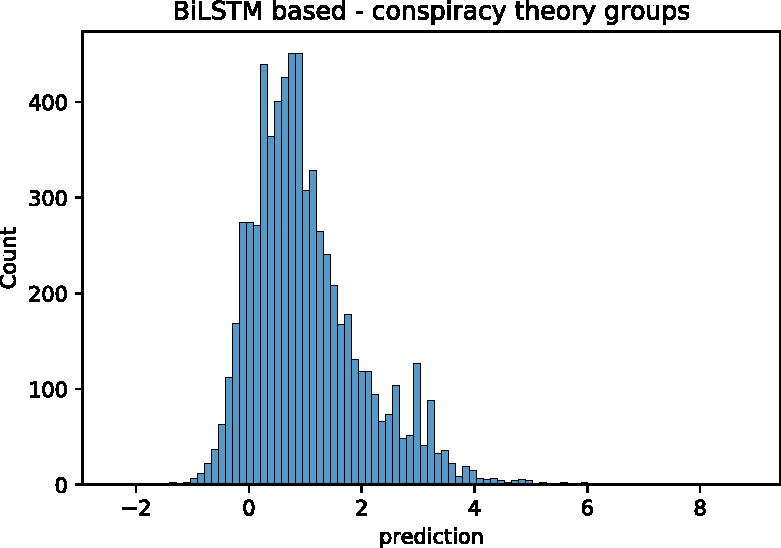
\includegraphics[width=.33\textwidth]{../report/figures/prediction_groups/bilstm_dist.pdf}
      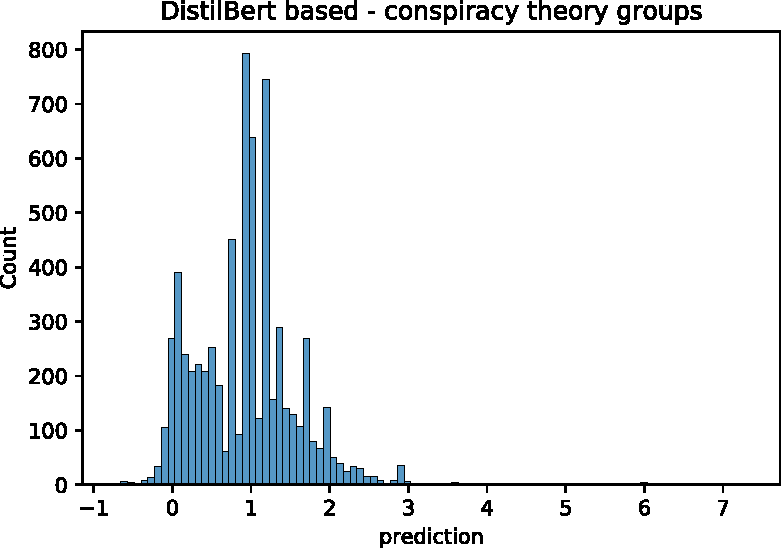
\includegraphics[width=.32\textwidth]{../report/figures/prediction_groups/distil_bert_dist.pdf}
      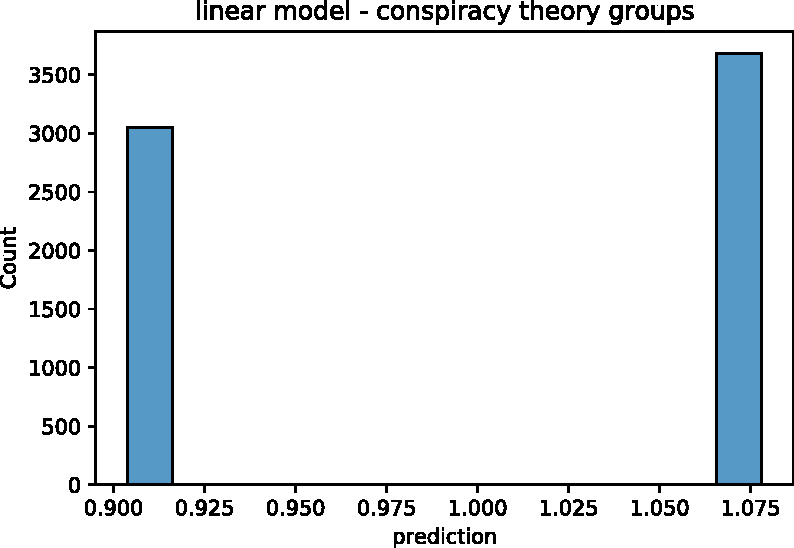
\includegraphics[width=.33\textwidth]{../report/figures/prediction_groups/linear_model_prediction_dist.pdf}
      \caption{distribution of the model's score variable prediction for the conspiracy theory group dataset}
      \label{fig:dist-prediction-groups}
  \end{figure}
\end{frame}

\begin{frame}
  \frametitle{Results}
  \begin{figure}[tb]
      \centering
      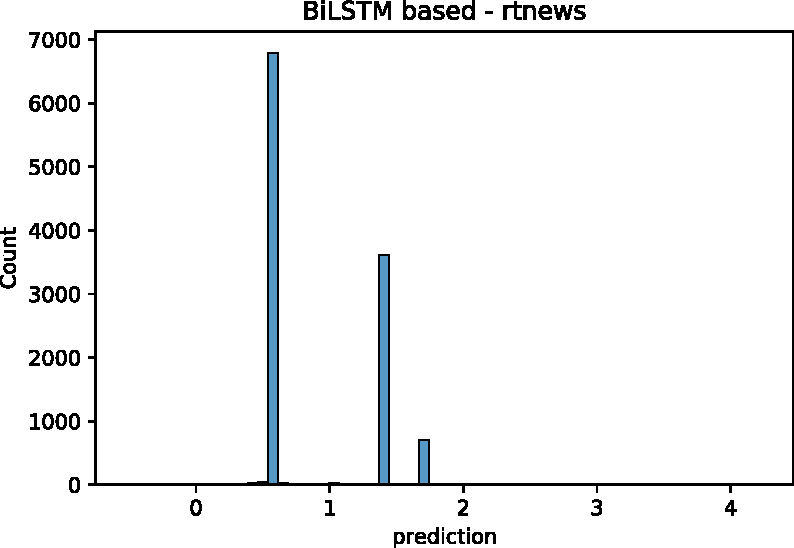
\includegraphics[width=.33\textwidth]{../report/figures/prediction_rtnews/bilstm_dist.pdf}
      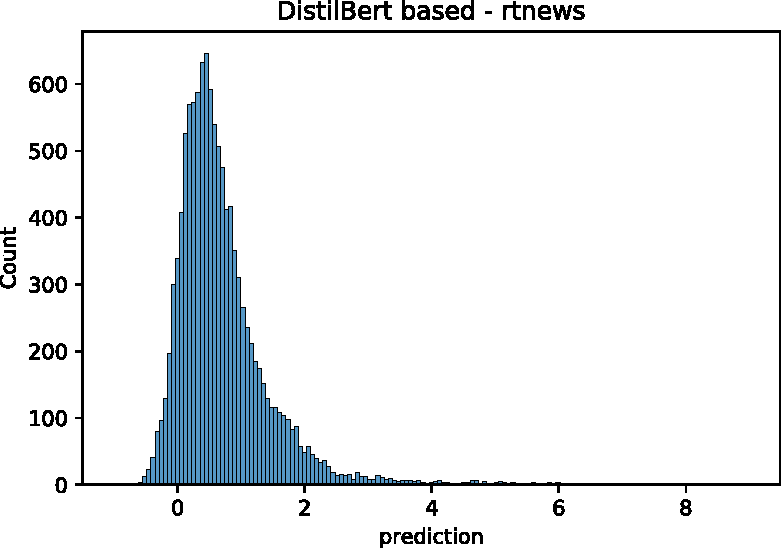
\includegraphics[width=.32\textwidth]{../report/figures/prediction_rtnews/distil_bert_dist.pdf}
      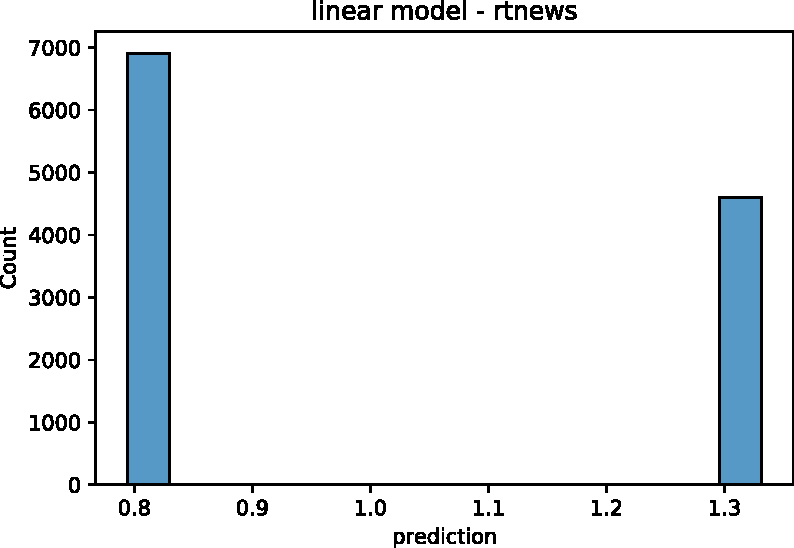
\includegraphics[width=.33\textwidth]{../report/figures/prediction_rtnews/linear_model_prediction_dist.pdf}
      \caption{distribution of the model's score variable prediction for the rtnews dataset}
      \label{fig:dist-prediction-rtnews}
  \end{figure}
\end{frame}

\begin{frame}
  \frametitle{Discussion}
  \begin{itemize}
    \item We could not outperform the baseline model
    \item The baseline model is already comprehensible for humans
  \end{itemize}
  \vspace*{2cm}
  \begin{itemize}
    \item Uniform distribution of reactions
    \item Use of other topics / groups
    \item No relation at all?
  \end{itemize}
\end{frame}


\begin{frame}
  \frametitle{Thank you for your attention}

  Feel free to ask questions!
\end{frame}

\begin{frame}[allowframebreaks]
  \frametitle{References}
  \nocite{*}
  \bibliography{literature}
\end{frame}


%%\addcontentsline{toc}{section}{Bibliography} 

\end{document}
